\section{光储充直流微电网系统建模}

为了深入探究光照突变、负载切入等多重扰动下直流微电网的暂态失稳机理，建立准确、合理且具备明确物理意义的系统级数学与仿真模型是后续研究的核心前提。

本章以光储充直流微电网为研究对象，采用模块化建模思想，分别对微电网中的四大核心物理单元进行数学推导与控制系统设计。首先，建立了光伏阵列的非线性输出模型及其配套的最大功率点跟踪（MPPT）控制策略；其次，构建了储能电池的等效电路模型及双向充放电控制架构；再次，详细推导了网侧逆变器在同步旋转 $dq$ 坐标系下的并网控制方程。最后，针对系统级暂态仿真中高频物理充电桩导致“维度灾难”的工程痛点，提出并详细论述了一种基于受控源的恒功率负载（CPL）等效降阶建模方法，为后续的高效大尺度暂态分析奠定了坚实的模型基础。

\subsection{光伏发电系统建模与控制}

光伏发电系统是直流微电网的主要能量来源之一，其输出功率受环境温度与光照强度（辐照度）的强烈制约，呈现出典型的非线性特征。为了实现光伏阵列的高效并网，通常需要通过DC/DC变换器（如Boost升压电路）接入直流母线，并配合相应的控制算法以维持最大功率输出。

\subsubsection{光伏电池等效数学模型}

太阳能光伏电池的物理本质是一个大面积的PN结，其将太阳辐射能直接转换为电能。在工程应用与系统级仿真中，为了兼顾计算精度与模型复杂度，通常采用经典的“单二极管五参数等效电路模型”来描述光伏电池的输出外特性。

该等效电路主要由一个光生电流源 $I_{ph}$、一个反向并联的二极管 $D$、一个等效并联电阻 $R_{sh}$ 以及一个等效串联电阻 $R_s$ 构成。
\begin{figure}[htbp]
    \centering
    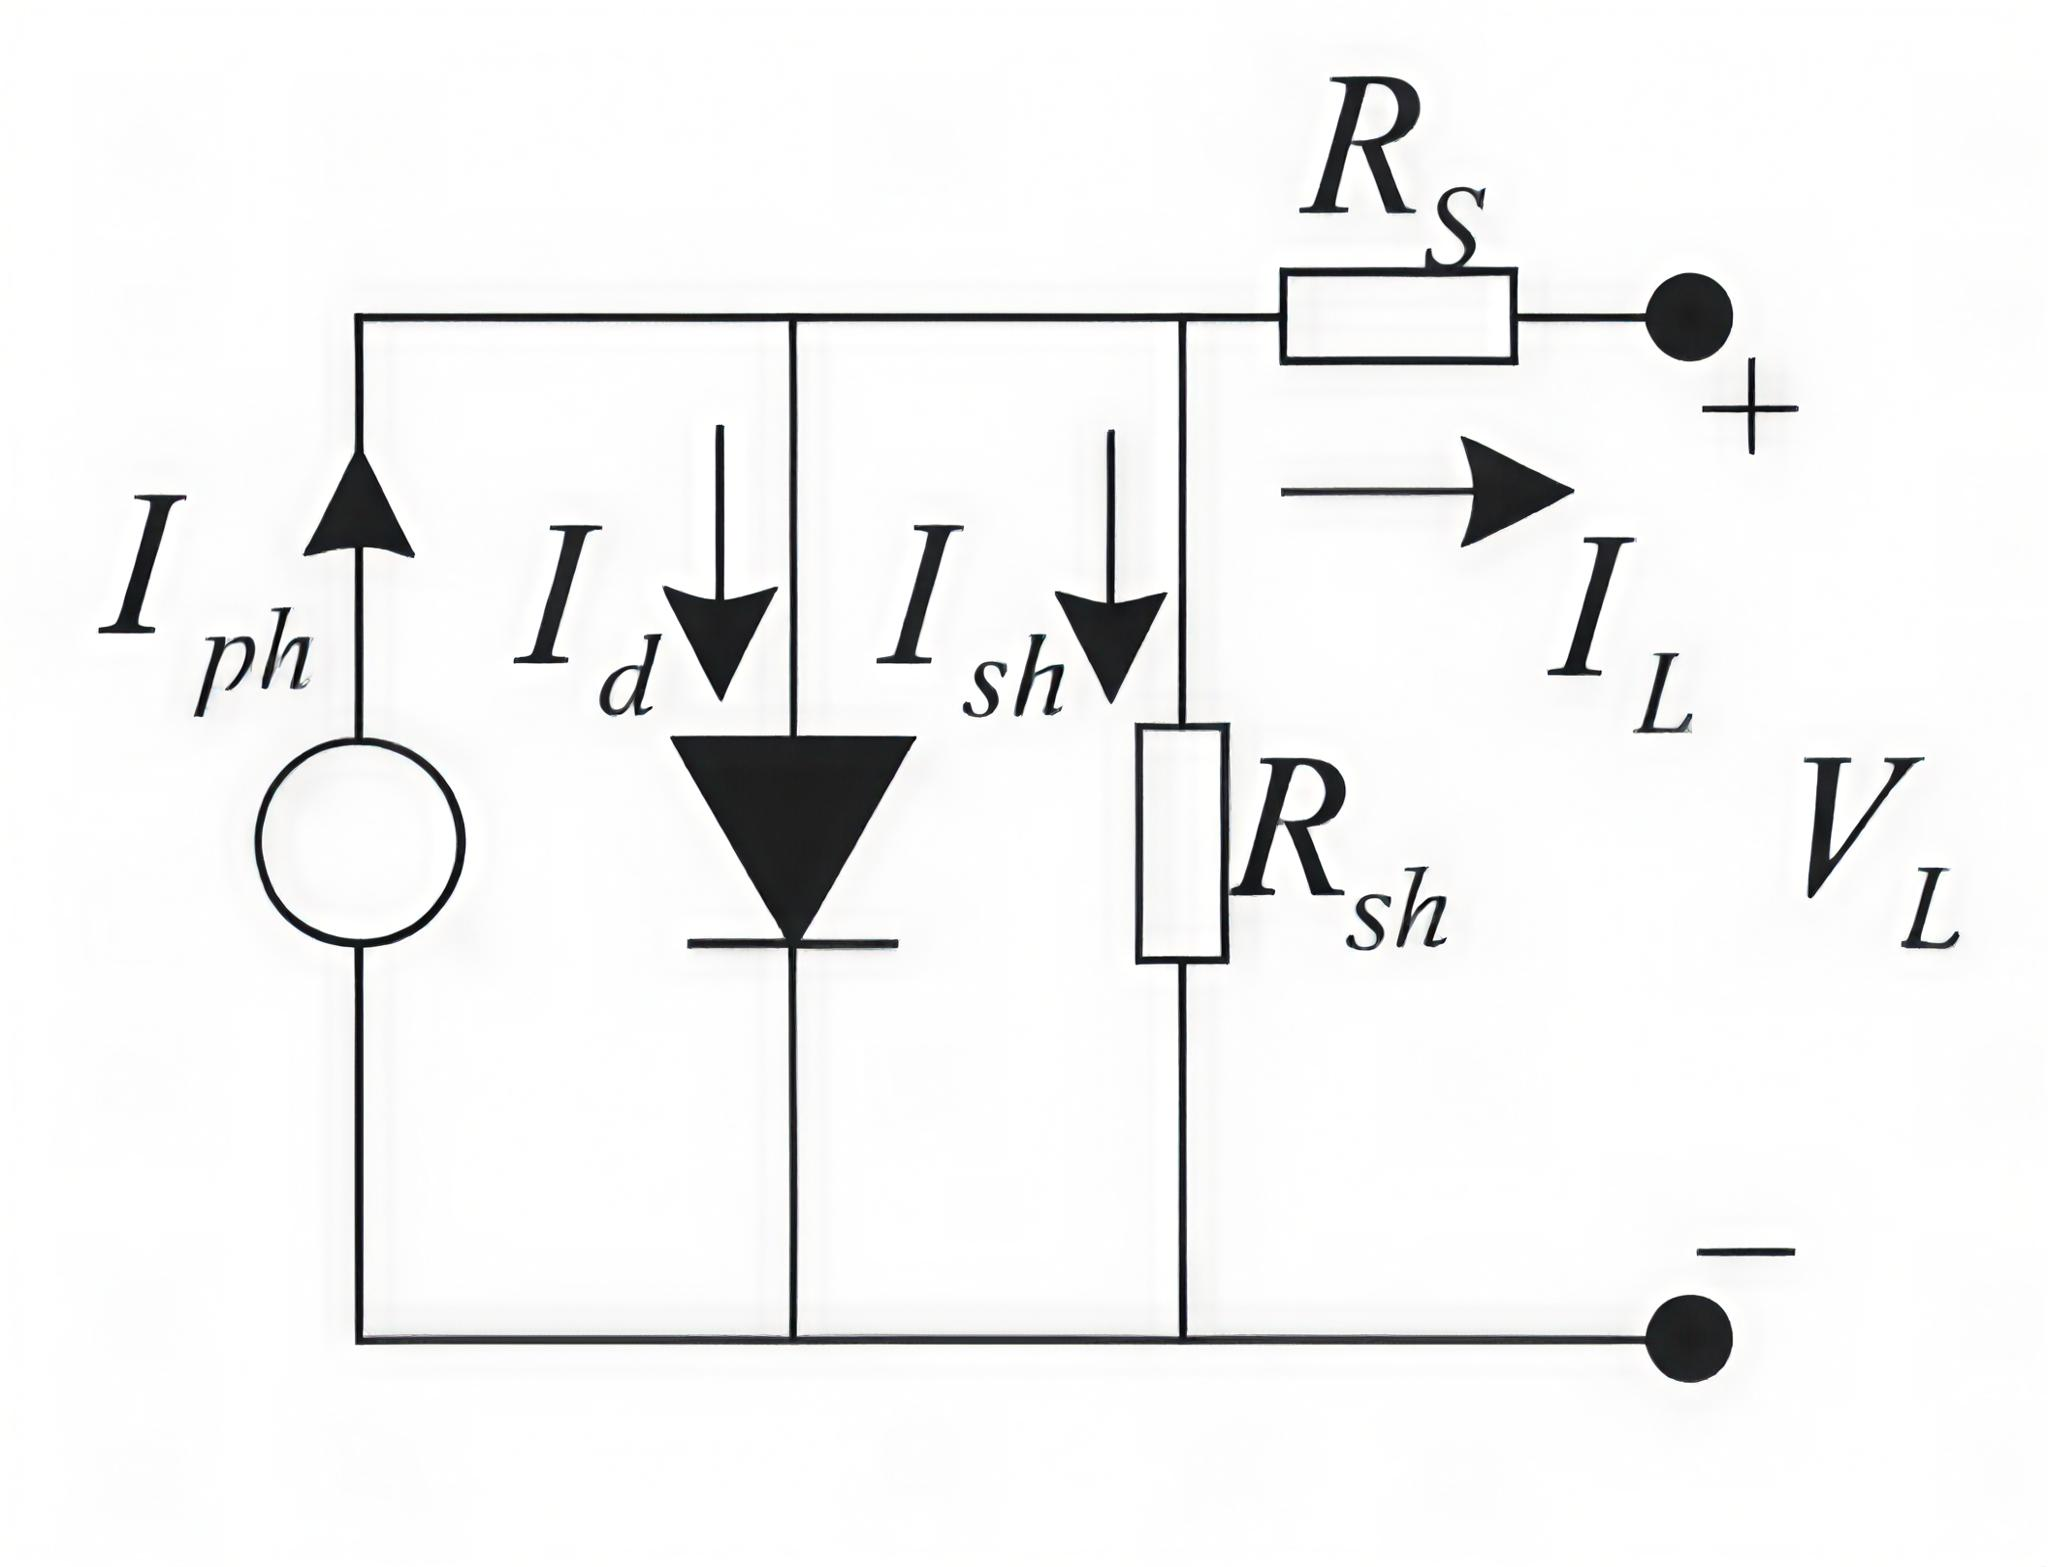
\includegraphics[width=0.6\textwidth]{figures/fig2_1_pv_model.png}
    \caption{光伏电池单二极管等效电路模型}
    \label{fig:pv_model}
\end{figure}
% TODO: 待插入单二极管等效电路图

根据基尔霍夫电流定律，可推导出光伏电池在任意光照与温度条件下的输出电流 $I$ 与端电压 $V$ 的非线性解析方程：
\begin{equation}
    I = I_{ph} - I_{d} - I_{sh}
\end{equation}
\begin{equation}
    I = I_{ph} - I_0 \left[ \exp\left( \frac{q(V + I R_s)}{A k T} \right) - 1 \right] - \frac{V + I R_s}{R_{sh}}
\end{equation}

式中各物理量的含义及其影响机制如下：
\begin{itemize}
    \item $I_{ph}$ 为光生电流（A），其大小与当前的光照强度（辐照度 $S$）成正比，是光伏电池有功出力的根本来源；
    \item $I_0$ 为二极管的反向饱和电流（A），受环境温度 $T$ 的影响极为显著；
    \item $q$ 为电子电荷常量（约 $1.602 \times 10^{-19}$ C）；
    \item $k$ 为玻尔兹曼常数（约 $1.381 \times 10^{-23}$ J/K）；
    \item $A$ 为二极管的理想因子，通常取值在 1 到 2 之间；
    \item $T$ 为PN结的绝对温度（K）；
    \item $R_s$ 为等效串联电阻（$\Omega$），代表半导体材料体电阻及金属接触电阻，其值虽然极小，但在大电流输出时会引起显著的电压跌落；
    \item $R_{sh}$ 为等效并联电阻（$\Omega$），表征PN结边缘的漏电流效应，通常阻值极大。
\end{itemize}

上述超越方程由于存在指数项且电压电流相互耦合，无法直接求出解析解。在实际的Simulink系统级仿真中，通常利用牛顿-拉夫逊（Newton-Raphson）等数值迭代算法求解该模型，从而准确拟合出不同环境条件下的 P-V 与 I-V 非线性输出特性曲线。


\subsubsection{Boost变换器与MPPT控制策略}

由于单体光伏电池的输出电压极低，且其输出功率随外部环境剧烈波动，光伏阵列通常无法直接并入高压直流母线。因此，在光伏阵列与直流母线之间级联一个 Boost 升压变换器是必不可少的。Boost 变换器不仅承担着升压与能量传递的任务，更关键的是作为执行机构，通过调节全控型开关器件（如 IGBT）的占空比 $D$，强制改变光伏阵列的输出工作点，从而实现最大功率点跟踪（MPPT）。

Boost 变换器的主电路拓扑主要由输入滤波电容、储能电感、全控型开关管、续流二极管以及输出滤波电容构成。在连续导通模式（CCM）下，其输入电压 $V_{in}$（即光伏阵列端电压）与输出直流母线电压 $V_{out}$ 满足如下理想关系：
\begin{equation}
    V_{out} = \frac{V_{in}}{1 - D}
\end{equation}
其中，$D$ 为开关管的导通占空比（$0 \le D < 1$）。由上式可知，通过改变占空比 $D$，可以灵活控制光伏阵列的输出电压 $V_{in}$，使其始终运行在 P-V 曲线的顶点。

为了在复杂的环境变化中实时锁定光伏阵列的最大功率点，本文系统采用了控制精度极高的\textbf{电导增量法（Incremental Conductance, INC）}作为 MPPT 控制算法。相比于传统的扰动观察法（P\&O），电导增量法能够有效避免在最大功率点附近的振荡，且对光照突变具有更优异的动态响应速度。

电导增量法的核心数学思想在于对光伏电池的 P-V 曲线进行求导分析。在最大功率点（MPP）处，功率 $P$ 对电压 $V$ 的导数必然为零，即：
\begin{equation}
    \frac{dP}{dV} = 0
\end{equation}
由于功率 $P = V \cdot I$，对其展开求导可得：
\begin{equation}
    \frac{dP}{dV} = \frac{d(V \cdot I)}{dV} = I + V \frac{dI}{dV} = 0
\end{equation}
进一步移项，即可得到判断最大功率点的核心判据：
\begin{equation}
    \frac{dI}{dV} = -\frac{I}{V}
\end{equation}
式中，$\frac{I}{V}$ 定义为光伏阵列的瞬时电导，$\frac{dI}{dV}$（离散化后即为 $\frac{\Delta I}{\Delta V}$）定义为电导的增量。

在实际仿真控制逻辑中，MPPT 控制器通过实时采样光伏阵列当前的输出电压 $V(k)$ 与电流 $I(k)$，并计算出电压变化量 $\Delta V = V(k) - V(k-1)$ 与电流变化量 $\Delta I = I(k) - I(k-1)$，进而执行以下核心判断逻辑：
\begin{itemize}
    \item 若 $\frac{\Delta I}{\Delta V} > -\frac{I}{V}$，说明当前工作点位于 MPP 的左侧（$dP/dV > 0$），需减小占空比 $D$ 以提升光伏输出电压；
    \item 若 $\frac{\Delta I}{\Delta V} < -\frac{I}{V}$，说明当前工作点位于 MPP 的右侧（$dP/dV < 0$），需增大占空比 $D$ 以降低光伏输出电压；
    \item 若 $\frac{\Delta I}{\Delta V} = -\frac{I}{V}$，说明已准确锁定最大功率点，保持当前占空比 $D$ 不变。
\end{itemize}

最终，MPPT 算法输出的占空比指令 $D$ 经过 PWM 调制模块，生成高频开关信号驱动 Boost 变换器中的 IGBT，从而在“源”侧建立起坚实的第一道抗扰动防线。
\begin{figure}[htbp]
    \centering
    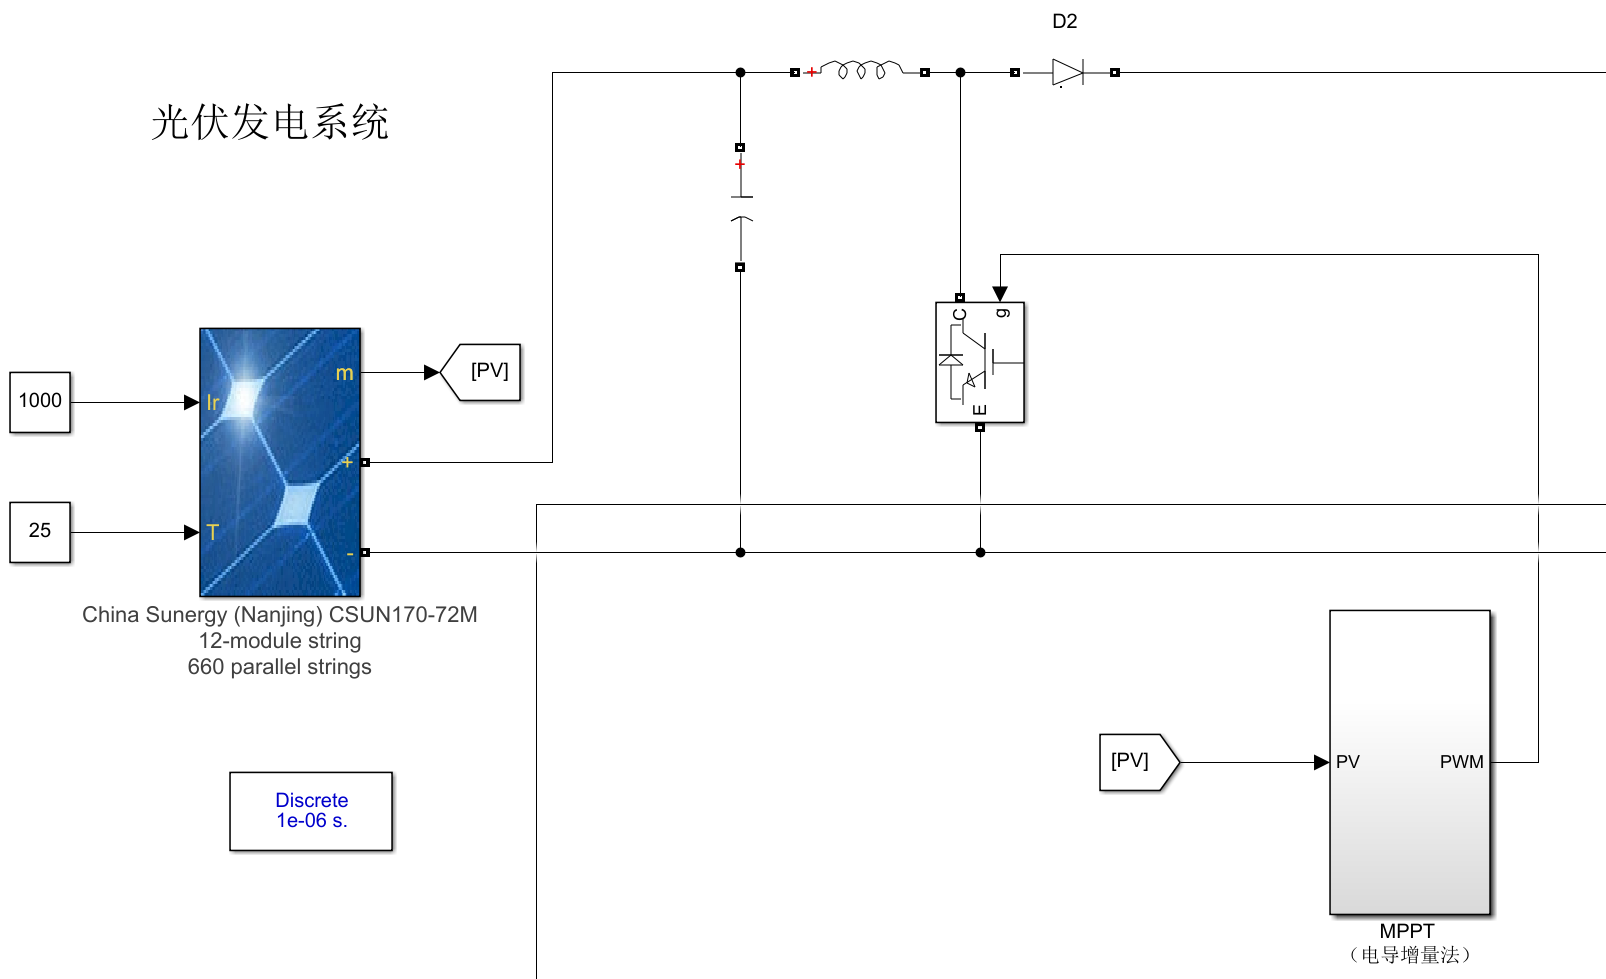
\includegraphics[width=0.85\textwidth]{figures/fig2_2_pv_simulink.png}
    \caption{光伏发电系统及Boost升压电路仿真拓扑}
    \label{fig:pv_simulink}
\end{figure}
% TODO: 待插入包含 PV Array、Boost 电路与电导增量 MPPT 模块的仿真拓扑截图

\subsection{储能电池系统建模与控制}

在光储充直流微电网中，储能系统（ESS）扮演着极其关键的“能量缓冲池”角色。在并网运行模式下，当系统遭遇光伏出力突变或大功率快充负荷突加等剧烈扰动时，储能系统需要具备极快的动态响应能力，通过吸收或释放功率来平抑直流母线电压的暂态波动，从而保障微电网的安全稳定运行。

\subsubsection{电池本体等效电路模型}

实际的锂离子电池内部发生着复杂的电化学反应。在进行系统级暂态仿真时，为了准确表征电池在大电流充放电过程中的动态电压响应特性，本文采用二阶 Thevenin 等效电路模型对电池本体进行降阶建模。

Thevenin 模型将电池等效为一个理想电压源与电阻、电容网络的组合。其输出端电压 $V_{bat}$ 的解析表达式为：
\begin{equation}
    V_{bat} = E_0 - I_{bat} R_{in} - V_{p1} - V_{p2}
\end{equation}
式中，$E_0$ 为电池的开路电压，其值随电池的荷电状态（State of Charge, SOC）呈非线性变化；$I_{bat}$ 为电池的充放电电流（规定放电为正）；$R_{in}$ 为电池的欧姆内阻，主要引起瞬间的电压跌落；$V_{p1}$ 与 $V_{p2}$ 分别为两个 RC 极化网络两端的电压，用于模拟电池内部电化学极化和浓差极化所带来的缓慢动态响应过程。

通过 Thevenin 模型，仿真系统能够高度逼真地复现出储能电池在面对 CPL 负阻抗冲击时，因大电流输出而产生的端电压暂态跌落现象。
\begin{figure}[htbp]
    \centering
    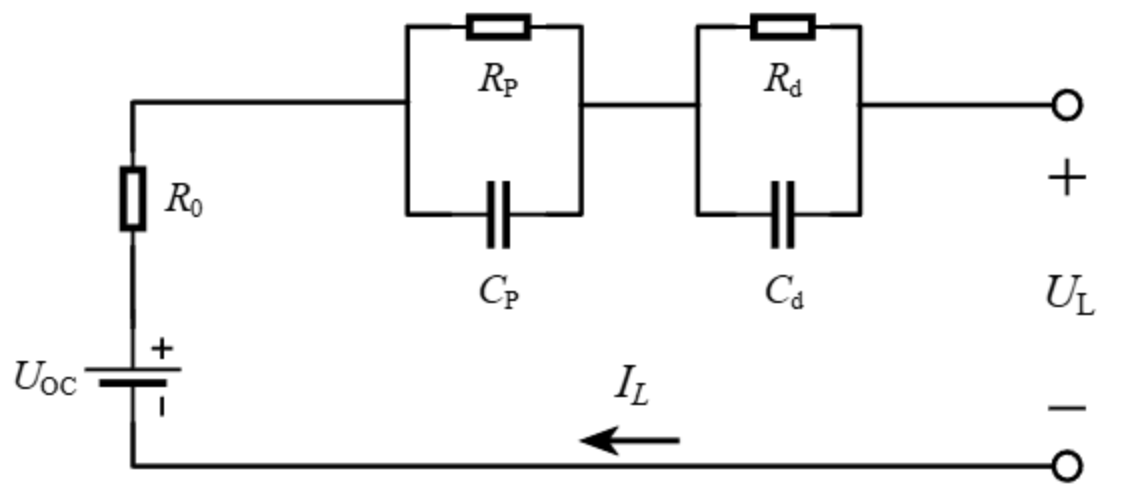
\includegraphics[width=0.6\textwidth]{figures/fig2_3_battery_model.png}
    \caption{储能电池二阶 Thevenin 等效电路模型}
    \label{fig:battery_model}
\end{figure}
\subsubsection{双向 Buck-Boost 变换器及双闭环控制}

储能电池的端电压通常低于直流母线电压，且需具备双向能量流动的能力。因此，储能系统通过一个非隔离型双向 Buck-Boost DC/DC 变换器接入直流母线。当母线功率富余时，变换器工作在 Buck 降压模式，为电池充电；当母线功率短缺（如大功率充电桩突加）时，变换器工作在 Boost 升压模式，电池向母线放电。

为了实现对直流母线电压的精确钳位与快速暂态支撑，储能变换器采用了经典的“电压外环 - 电流内环”双闭环 PI（比例-积分）控制策略。

% TODO: 待插入储能双闭环控制结构框图/Simulink截图

\textbf{1. 电压外环控制}

电压外环的主要目标是维持直流母线电压稳定。控制器实时采集直流母线实际电压 $V_{dc}$，并与系统设定的参考电压 $V_{dc\_ref}$ 进行比较。其误差信号 $e_v$ 经过外环 PI 控制器调节后，输出电池的参考指令电流 $I_{ref}$：
\begin{equation}
    I_{ref} = K_{pv} (V_{dc\_ref} - V_{dc}) + K_{iv} \int (V_{dc\_ref} - V_{dc}) dt
\end{equation}
式中，$K_{pv}$ 和 $K_{iv}$ 分别为电压外环的比例与积分增益。当 CPL 突加导致 $V_{dc}$ 跌落时，外环会迅速输出一个极大的正向电流指令 $I_{ref}$，命令电池全力放电。

\textbf{2. 电流内环控制}

电流内环的目标是使电池的实际电流 $I_{bat}$ 无静差地快速跟踪外环下发的指令电流 $I_{ref}$。内环 PI 控制器的响应带宽通常设计为外环带宽的 5 到 10 倍，以保证系统的暂态稳定性。其控制方程为：
\begin{equation}
    D_{duty} = K_{pi} (I_{ref} - I_{bat}) + K_{ii} \int (I_{ref} - I_{bat}) dt
\end{equation}
式中，$K_{pi}$ 和 $K_{ii}$ 为电流内环的比例与积分增益；$D_{duty}$ 为最终输出的占空比信号。该信号送入 PWM 发生器，生成互补的驱动脉冲控制双向变换器中的上下桥臂开关管。

通过这种严密的双闭环控制架构，储能系统能够在毫秒级尺度内响应大扰动，为微电网的暂态稳定性构筑了最核心的物理屏障。
\begin{figure}[!htbp]
    \centering
    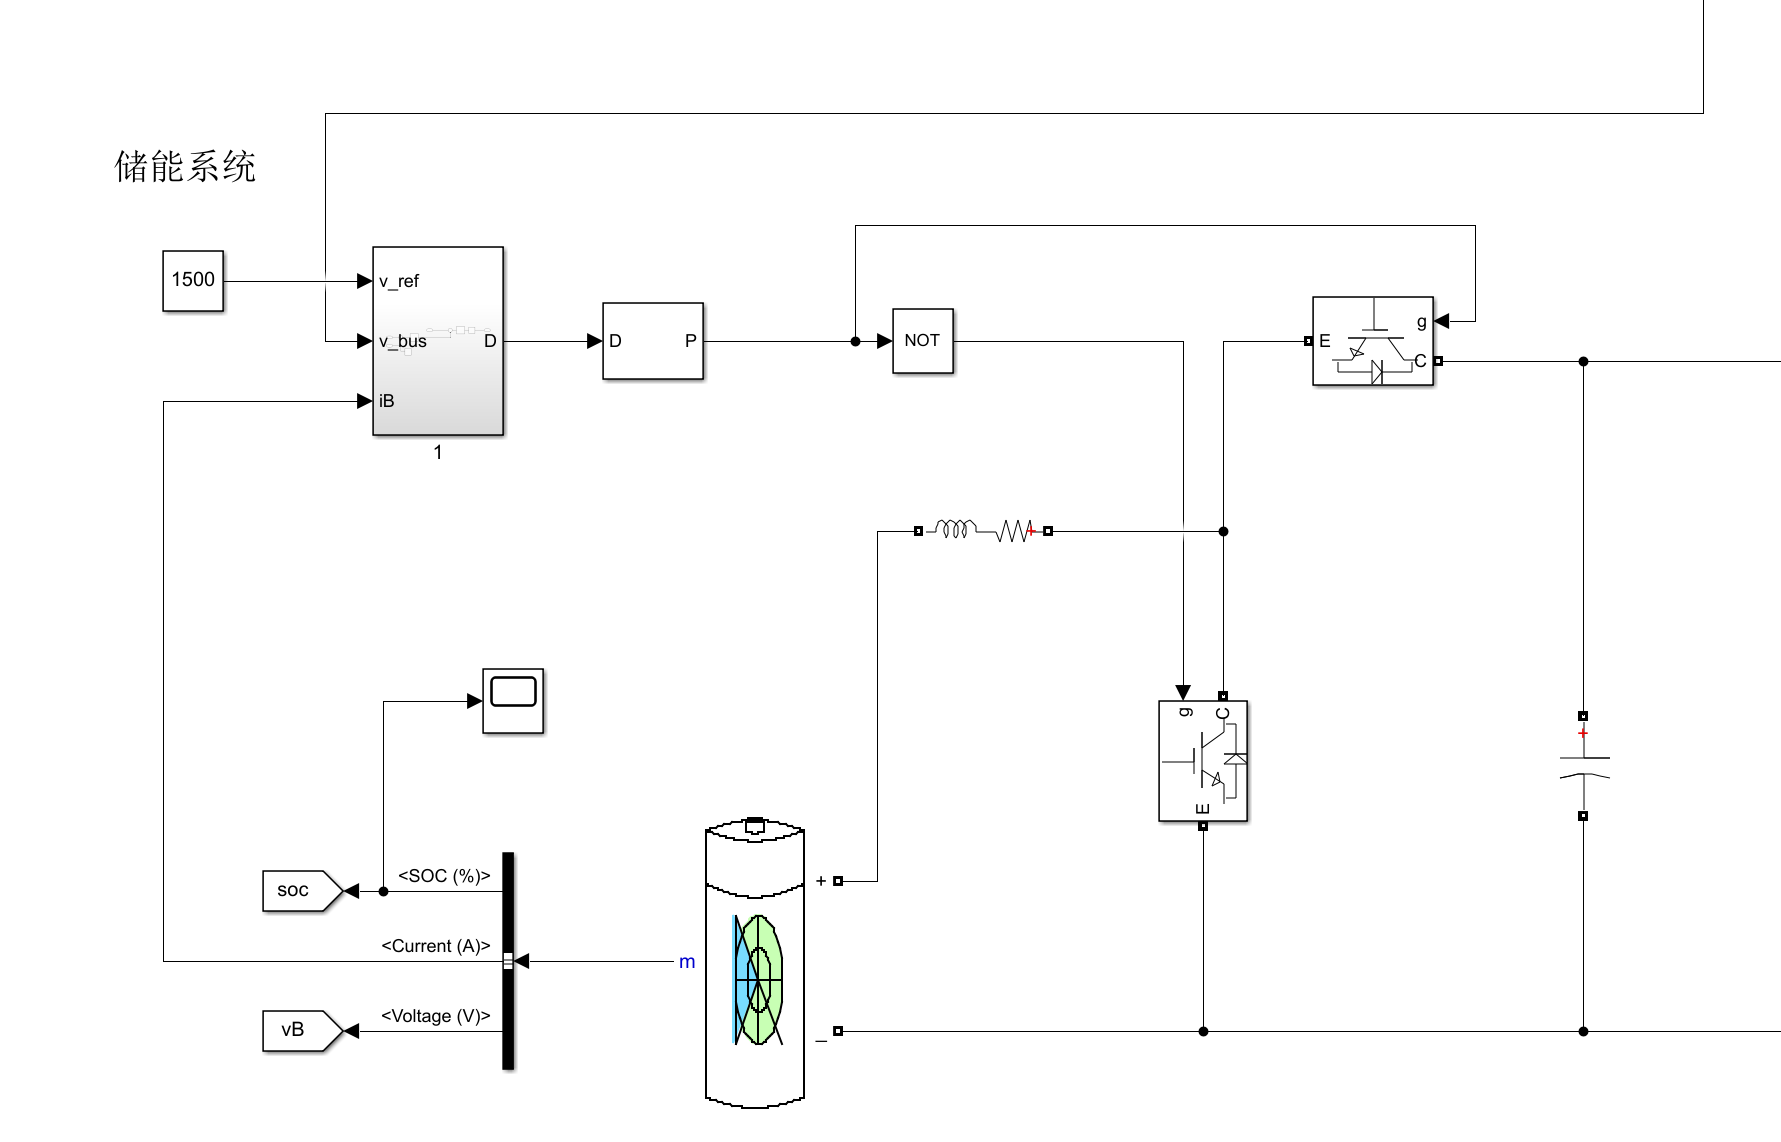
\includegraphics[width=0.85\textwidth]{figures/fig2_4_battery_simulink.png}
    \caption{储能双向变换器及双闭环控制仿真拓扑}
    \label{fig:battery_simulink}
\end{figure}

\subsubsection{电池容量衰退经验预测模型}

在光储充电站的长期优化运行中，储能电池的频繁充放电会导致不可逆的容量衰退，这构成了系统运行成本的重要组成部分。由于物理化学衰退机理极其复杂且时间尺度极长，本文在系统级建模中采用基于安时吞吐量（Ah-throughput）的半经验寿命衰退模型。

电池的容量衰退量与其工作温度、放电深度（DOD）及充放电倍率密切相关。为了便于后续的经济性优化调度，将其单次充放电循环引起的衰减折算为等效经济成本：
\begin{equation}
    C_{deg} = \frac{C_{bat\_cost}}{N_{cycle}(DOD)}
\end{equation}
式中，$C_{deg}$ 为单次循环的衰退成本，$C_{bat\_cost}$ 为电池初始投资成本，$N_{cycle}(DOD)$ 为特定放电深度下的最大循环寿命，通常由电池厂家提供的拟合曲线确定。该数学模型为后续的系统综合效益优化策略提供了核心的成本约束边界。

\subsection{网侧逆变器建模与并网控制}

网侧逆变器（Grid-Tied Inverter）是直流微电网与外部交流配电网进行能量交互的核心枢纽。在并网运行模式下，逆变器不仅需要维持高质量的并网电流波形，还需根据直流微电网内部的功率余缺，实现有功功率与无功功率的独立调节（PQ 控制）。

\subsubsection{逆变器主电路拓扑与数学模型}

本文系统采用三相电压型全桥逆变器（Voltage Source Inverter, VSI）作为并网接口。为了滤除高频 PWM 开关动作产生的谐波，在逆变器输出端与大电网之间串联了 LCL 型滤波器。相比于单 L 或 LC 滤波器，LCL 滤波器在体积更小的前提下，对高频频段具有更优异的衰减特性。

假设大电网为理想的三相对称电压源，基于基尔霍夫电压定律，在静止的 abc 三相坐标系下，逆变器交流侧的动态数学方程可表示为：
\begin{equation}
    \begin{bmatrix} v_{a} \\ v_{b} \\ v_{c} \end{bmatrix} =
    L \frac{d}{dt} \begin{bmatrix} i_{a} \\ i_{b} \\ i_{c} \end{bmatrix} +
    R \begin{bmatrix} i_{a} \\ i_{b} \\ i_{c} \end{bmatrix} +
    \begin{bmatrix} e_{a} \\ e_{b} \\ e_{c} \end{bmatrix}
\end{equation}
式中，$v_{a}, v_{b}, v_{c}$ 为逆变器桥臂输出的交流相电压；$i_{a}, i_{b}, i_{c}$ 为并网线电流；$e_{a}, e_{b}, e_{c}$ 为大电网侧的三相电压；$L$ 和 $R$ 分别为 LCL 滤波器的等效电感与等效串联电阻。

上述方程中的交流量随时间呈正弦规律变化，难以利用传统的 PI 控制器实现无静差跟踪。因此，必须引入坐标变换理论对其进行解耦降阶。

\begin{figure}[htbp]
    \centering
    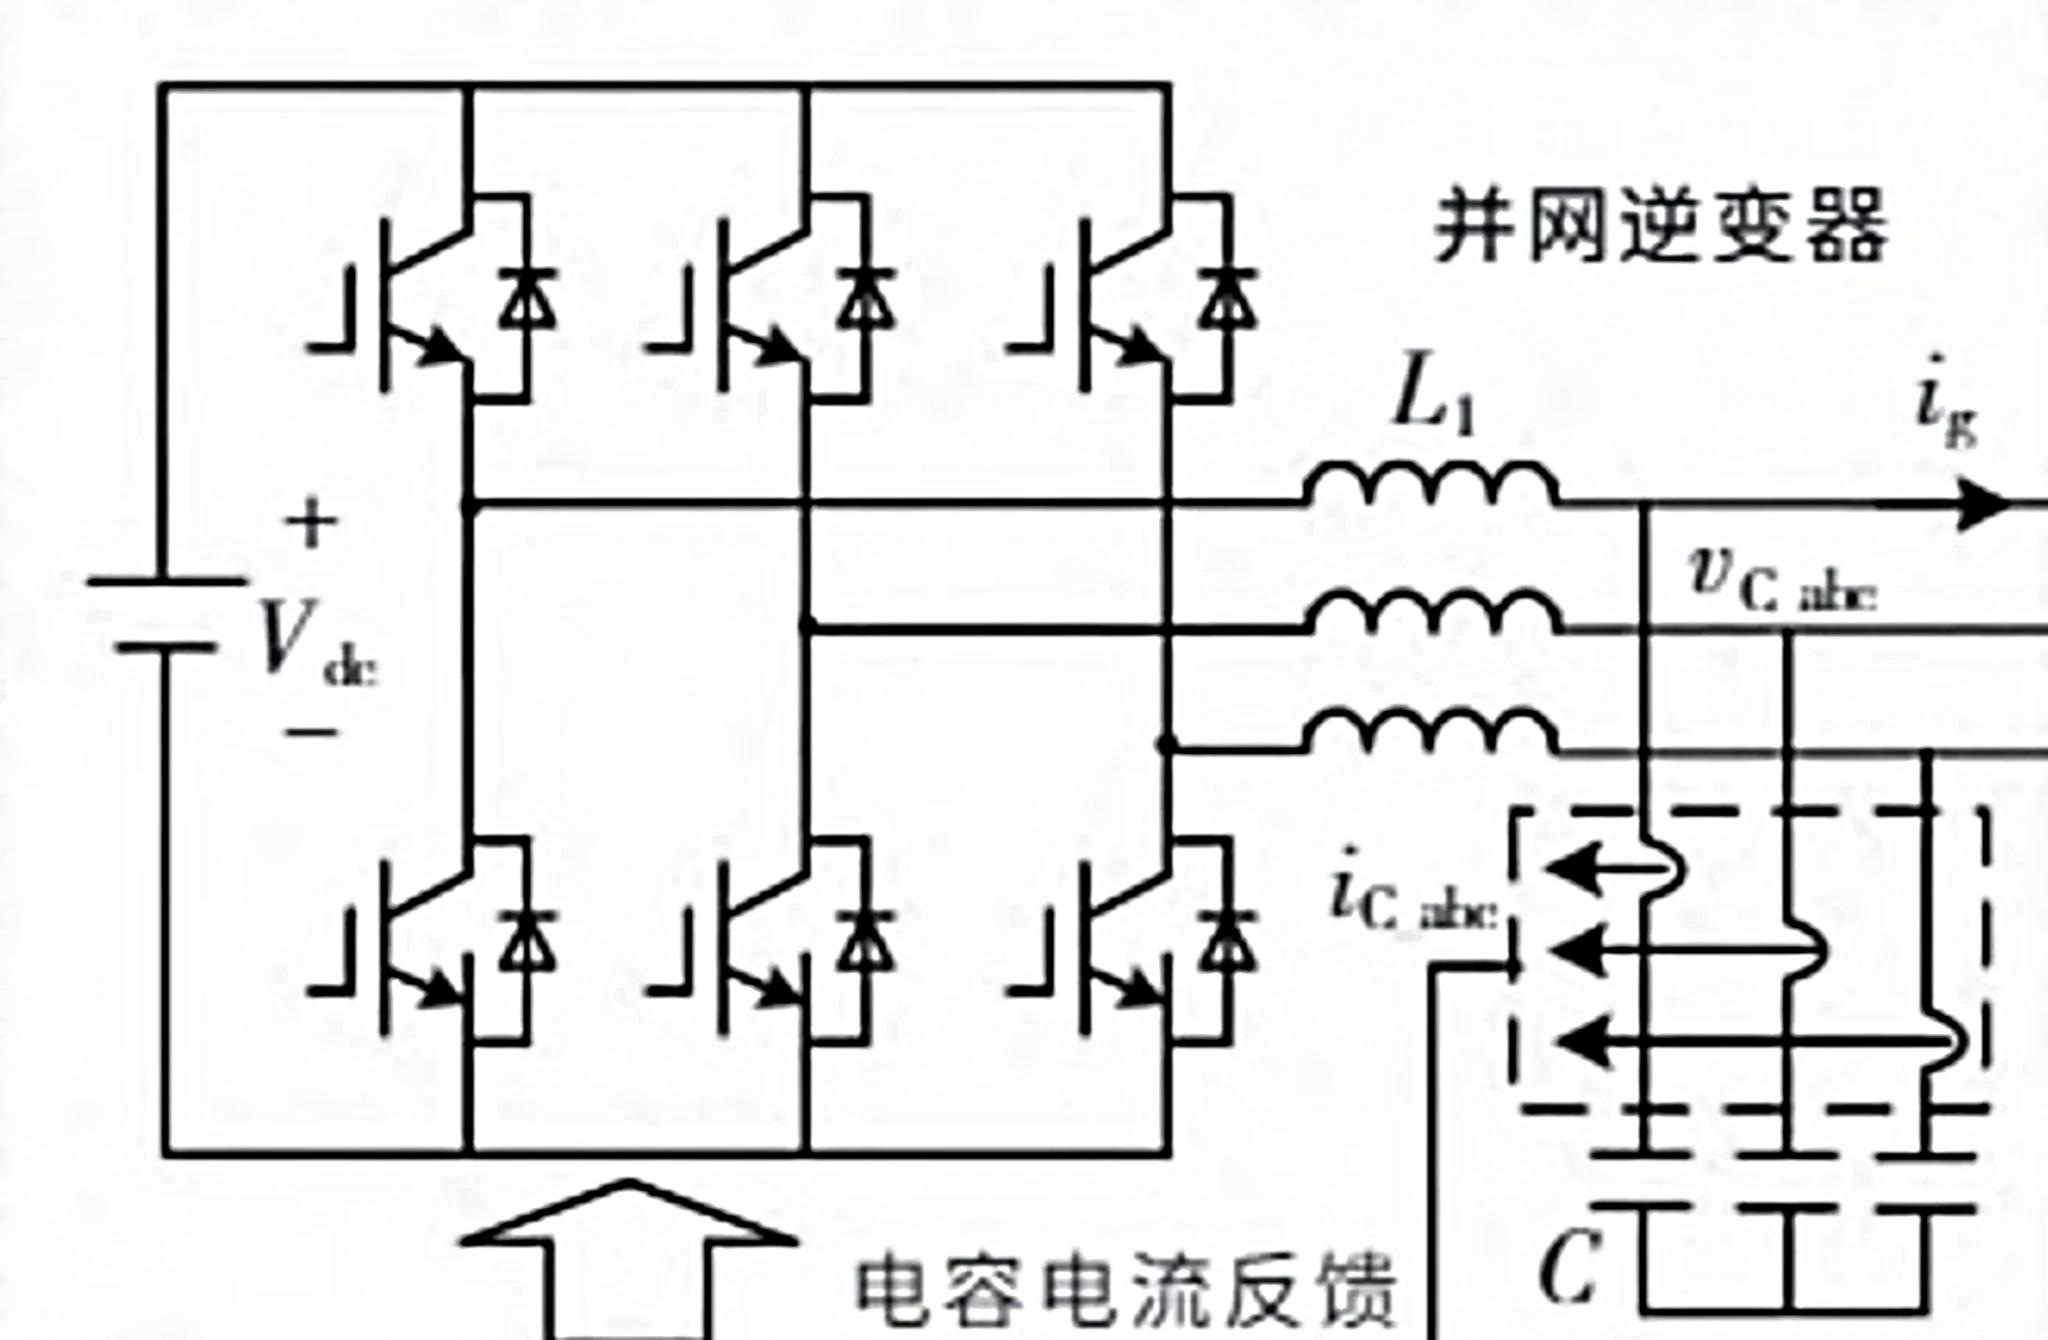
\includegraphics[width=0.65\textwidth]{figures/fig2_5_inverter_topology.png}
    \caption{三相并网逆变器及 LCL 滤波器等效拓扑}
    \label{fig:inverter_topology}
\end{figure}

\subsubsection{基于 $dq$ 坐标系的解耦控制策略}

为了实现对有功电流和无功电流的独立控制，本文采用基于电网电压定向的矢量控制策略。首先，通过锁相环（Phase-Locked Loop, PLL）实时获取电网电压的相位角 $\theta$。随后，利用 Park 变换，将 abc 静止坐标系下的交流量投影到以电网基波角频率 $\omega$ 同步旋转的 $dq$ 坐标系中。

在 $dq$ 旋转坐标系下，原本随时间交变的电流量转化为了直流量。此时，逆变器的数学模型解耦为：
\begin{equation}
    \begin{cases}
        v_{d} = L \frac{di_{d}}{dt} + R i_{d} - \omega L i_{q} + e_{d} \\
        v_{q} = L \frac{di_{q}}{dt} + R i_{q} + \omega L i_{d} + e_{q}
    \end{cases}
\end{equation}
式中，下标 $d$ 和 $q$ 分别代表直轴（有功分量）和交轴（无功分量）。可以发现，$d$ 轴和 $q$ 轴方程中存在相互耦合的交叉项（$-\omega L i_{q}$ 和 $+\omega L i_{d}$），这会导致有功和无功的调节相互干扰。

为了消除这种耦合效应，控制系统在传统的电流 PI 闭环基础上，引入了电网电压前馈与交叉解耦补偿项。最终，逆变器输出的电压指令方程可设计为：
\begin{equation}
    \begin{cases}
        v_{d}^* = (K_{pi} + \frac{K_{ii}}{s}) (i_{d\_ref} - i_{d}) - \omega L i_{q} + e_{d} \\
        v_{q}^* = (K_{pi} + \frac{K_{ii}}{s}) (i_{q\_ref} - i_{q}) + \omega L i_{d} + e_{q}
    \end{cases}
\end{equation}

在并网运行（PQ 控制）模式下，$d$ 轴指令电流 $i_{d\_ref}$ 由上级能量管理系统根据直流母线功率需求下发（或由直流电压外环生成），而 $q$ 轴指令电流 $i_{q\_ref}$ 通常设为 0，以保证系统运行在单位功率因数状态（即只传输有功功率，不传输无功功率）。计算出的 $v_{d}^*$ 和 $v_{q}^*$ 经反 Park 变换（$dq$ 转 abc）后，送入空间矢量脉宽调制（SVPWM）模块，驱动逆变器安全稳定运行。

\begin{figure}[htbp]
    \centering
    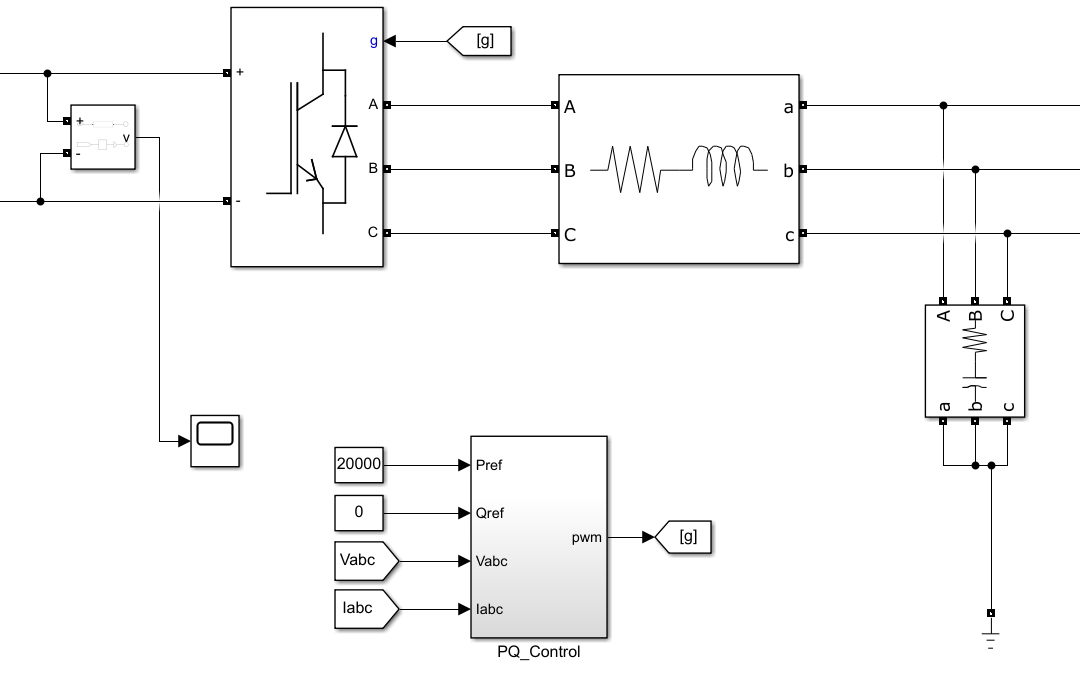
\includegraphics[width=0.85\textwidth]{figures/fig2_6_inverter_simulink.png}
    \caption{逆变器并网控制系统 Simulink 仿真模型}
    \label{fig:inverter_simulink}
\end{figure}


\subsection{充电桩负载等效降阶建模（恒功率负载特性）}

在光储充电站直流微电网中，电动汽车充电桩是系统最主要的负载。实际的大功率直流快充桩内部通常采用全桥 LLC 谐振变换器等多级高频隔离拓扑。这是本文系统级暂态仿真建模中最核心的挑战。

\subsubsection{高频物理模型引发的维度灾难}

在进行微电网系统级大扰动暂态分析时，研究的时间尺度通常在毫秒至秒级，重点关注的是各分布式电源之间的宏观能量流动与直流母线电压的低频动态演变。而物理充电桩内部的开关频率通常高达几十甚至上百千赫兹。

如果在系统级仿真中直接采用包含真实 IGBT 和高频变压器的物理级开关模型，一方面会引入海量与宏观稳定性无关的高频开关纹波，掩盖系统真实的低频暂态物理过程；另一方面，由于仿真步长必须小于最小开关周期的几分之一（通常需设定在 1$\mu$s 以下），海量状态变量的非线性迭代会导致严重的“维度灾难（Dimensionality Curse）”与计算资源枯竭，极易引发仿真求解器的内存溢出与死锁。因此，在保留宏观外特性的前提下，对物理充电桩进行合理的降阶等效建模，是开展高效、精准暂态分析的关键科学基础。

\subsubsection{充电桩的恒功率负载（CPL）物理本质}

当电动汽车接入充电桩进行快速充电时，充电桩内部的高带宽闭环控制系统会严密调节输出电流与电压，力求向 EV 电池输出恒定的充电功率 $P$。由于充电桩的控制带宽远高于直流微电网系统级的电压调节带宽，因此在微电网宏观尺度看来，充电桩表现出典型的恒功率负载外特性。

对于恒功率负载，其消耗的功率 $P$ 保持恒定。根据电学基本定律 $P = V \cdot I$，其端口电流 $I$ 与端口电压 $V$ 的关系可表示为：
\begin{equation}
    I = \frac{P}{V}
\end{equation}

对其进行求导，可得到 CPL 的增量阻抗解析表达式：
\begin{equation}
    R_{inc} = \frac{dV}{dI} = \frac{d}{dI} \left( \frac{P}{I} \right) = -\frac{P}{I^2} = -\frac{V^2}{P}
\end{equation}

由上式可知，CPL 的增量阻抗 $R_{inc}$ 始终为负值。这在物理上意味着：当直流母线电压 $V$ 受到扰动发生跌落时，为了维持恒定功率 $P$，负载会自动增大抽取电流 $I$；而增大的电流会进一步拉低母线电压，形成一种极其危险的反馈机制。这种独特的负阻抗特性极大地削弱了微电网的系统阻尼，是引发暂态失稳的根源。

\subsubsection{基于受控电流源的等效降阶建模方案}

为了在剥离高频开关动态的同时，完美复现 CPL 的宏观负阻抗冲击特性，本文提出了一种基于受控电流源的等效降阶建模方案。

该等效模型的核心控制逻辑如图 \ref{fig:cpl_model} 所示。系统首先通过电压测量模块实时采集直流母线电压 $V_{dc}$。在实际工程仿真中，直接采用 $I = P/V$ 逻辑会面临一个致命的数学奇点：在仿真启动瞬间（$t=0$）或母线发生极端短路故障时，母线电压 $V_{dc}$ 可能为 0 或极低，这将导致除法器分母为零，瞬间引发求解器崩溃（代数环死锁）。

为了解决这一难题并保证仿真的绝对稳定性，本文在电压前馈通路上设计了“一阶低通滤波与常数偏置”的隐式软启动机制。首先，采集到的母线电压经过时间常数为 $0.001s$ 的一阶低通滤波器，以平滑高频噪声带来的指令抖动；随后，在送入除法器分母前，叠加一个极小的正偏置常数（如 0.1 V）。这一数学处理不仅从根本上杜绝了除零奇点，而且在系统稳态（如母线运行于 750V）时，该偏置带来的计算误差不到万分之二，完全可以忽略不计。最终，经过安全处理的母线电压与阶跃功率指令相除，生成极其平滑且稳定的受控电流指令，高度还原了实际大功率快充桩的暂态功率抽取特性。

\subsection{基于蒙特卡洛模拟的电动汽车充电负荷建模}

为了在后续的优化运行策略中真实反映光储充电站的实际运行工况，必须建立符合用户出行规律的电动汽车（EV）充电负荷模型。由于单台 EV 的接入时间、初始荷电状态（SOC）和目标 SOC 均具有高度的随机性，本文采用蒙特卡洛（Monte Carlo）模拟方法生成充电站的宏观负荷曲线。

根据交通行为统计学数据，假设 EV 的到达时间 $t_{arr}$ 近似服从正态分布 $N(\mu_t, \sigma_t^2)$，初始接入时的 $SOC_{init}$ 服从另一个独立的正态分布 $N(\mu_{soc}, \sigma_{soc}^2)$。通过在 MATLAB 中利用伪随机数发生器对上述概率密度函数进行大量抽样，可得到每辆车的充电时长与功率需求：
\begin{equation}
    T_{charge} = \frac{(SOC_{target} - SOC_{init}) \cdot C_{EV}}{P_{charge} \cdot \eta}
\end{equation}
式中，$C_{EV}$ 为电动汽车电池容量，$P_{charge}$ 为充电桩额定功率，$\eta$ 为充电效率。将全天所有抽样车辆的充电功率在时间轴上进行叠加，即可得到具备高度随机性与真实物理意义的光储充电站 24 小时日前负荷预测曲线，为系统的长时尺度优化调度提供随机边界条件。